Un arbre binaire de recherche présente-t-il un avantage par rapport à une table de
hachage pour réaliser un \textit{Map} ? Pourquoi ? Et par rapport à une \textit{Skip List} ? \\
La forme d’un arbre binaire de recherche dépend-elle de l’ordre d’insertion des
clés ? La forme d’un arbre binaire de recherche dépend-elle de l’ordre de suppression
des clés ? Quelle est la complexité temporelle de l’insertion de $\textit{n}$ clés
identiques dans un arbre binaire de recherche initialement vide ? Quelle est la
propriété particulière des arbres binaires de recherche qui justifie l’intérêt d’autres
structures de données comme les Arbres AVL ou les Arbres (2,4) ? (Sundeep) 
\medskip

TODOOOOOOOOo

Pour ce qui concerne l'intérêt d'autres structures de données comme les Arbres AVL, il s'agit tout simplement d'essayer d'avoir une complexité temporelle logarithmique pour les principales opérations. Pour ce faire, la seule correction à effectuer consiste à ajouter une règle à la définition de l'arbre binaire de recherche pour maintenir une hauteur en logarithme pour l'arbre. La règle en question est la \textbf{propriété d'équilibre de l'hauteur}, celle-ci caractérise la structure d'un arbre binaire de recherche \textit{T} en termes des hauteurs de ses noeuds internes. Autrement dit, pour chaque noeud interne $\textit{v}$ de \textit{T}, les hauteurs des enfants de $\textit{v}$ diffèrents de 1 au maximum. Tout arbre binaire de recherche \textit{T} qui satisfait cette dernière propriété est appelé un \textbf{Arbre AVL\footnote{Ce nom provient de ses inventeurs, à savoir: Adel'son-Vel'skii et Landis}}. Une conséquence directe de cette propriété est qu'un sous-arbre d'un arbre AVL est d'office un arbre AVL. Une autre propriété est que la hauteur d'un arbre AVL pour stocker $\textit{n}$ entrées est $\textit{O}(log \textit{n})$.

\begin{figure} [!h]
\center
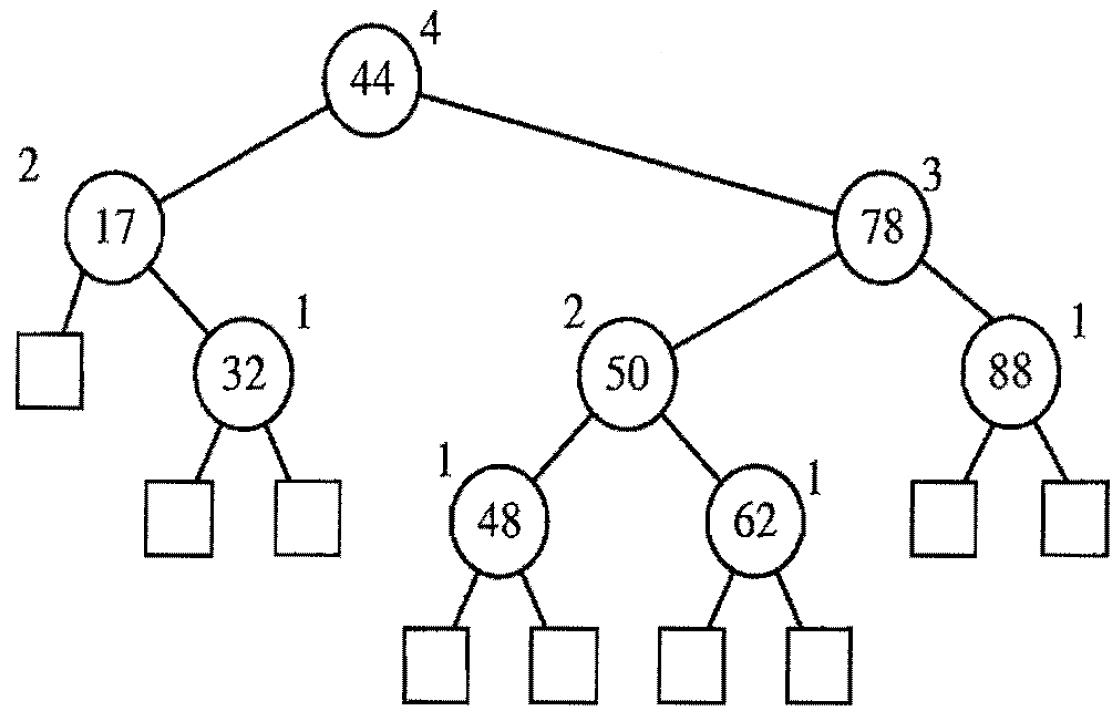
\includegraphics[scale=0.37]{AVL.png}
\caption{Exemple d'arbre AVL. Les clés des entrées sont mises à l'intérieur des noeuds et les hauteurs des noeuds sont indiquées à côté de ces derniers.}
\end{figure}

Arbres (2,4) TODOOOO		